% =============================================================================
% Lecture 11: Durable Execution
% Agentic Machine Learning Systems (Volume III), Chapter 11
% =============================================================================
% Thesis: to survive a crash without repeating an effect, the runtime records
% what it is about to do before doing it and rebuilds control state from the
% log without asking the model again.
% Hook and synthesis: the chapter's worksheet crash (the repair agent's test
% of r18 dispatched, then the worker dies), run for real for this lecture: a
% Temporal workflow whose worker was killed with SIGKILL during the test, and
% 30 restarts of the same task from its original prompt on a local model.
%
% Build: make deck V=3 D=11_durable_execution   (figures: images/make_figs.py)
% Plan:  lecture_map.yml in this folder.
% Numbers: images/calcs.py prints every derived value; sources named there.
% =============================================================================

\documentclass[aspectratio=169, 12pt]{beamer}
\usepackage{../../assets/beamerthememlsys}
\mlsyssetup{
  volume={Volume III},
  chapter={Chapter 11},
  chaptertitle={Durable Execution},
  layer=runtime,
  logo={../../assets/img/logo-mlsysbook.png},
  instlogo={../../assets/img/logo-harvard.png},
}
\usepackage[T1]{fontenc}
\usepackage[scaled=0.9]{helvet}
\usepackage{courier}
% Code and real tool output: Inconsolata is narrower than Courier.
\usepackage[varqu,scaled=0.95]{zi4}
\renewcommand{\familydefault}{\sfdefault}
\usepackage{booktabs,amsmath}
\usetikzlibrary{arrows.meta,positioning}
\graphicspath{{images/}}
% Generated by calcs.py. Do not edit; edit calcs.py and rerun it.
\defval{rs_n}{30}
\defval{rs_temp}{0.8}
\defval{rs_distinct}{8}
\defval{rs_read}{16}
\defval{rs_grep}{9}
\defval{rs_tests}{5}
\defval{rs_n0}{30}
\defval{rs_distinct0}{1}
\defval{rs_distinct0_words}{one}
\defval{metr_last_h}{17}
\defval{res_usd}{0.50}
\defval{cr_calls}{1}
\defval{cr_launches}{2}
\defval{cr_second_s}{3.9}
\defval{ack_n}{300}
\defval{ack_bytes}{512}
\defval{ack_write}{0.024}
\defval{ack_fsync}{0.043}
\defval{ack_full}{3.0}
\defval{ack_ratio}{70}
\defval{gc_kmin}{1}
\defval{gc_kmax}{64}
\defval{gc_flush_lo}{3}
\defval{gc_flush_hi}{3.6}
\defval{gc_per_hi}{3.1}
\defval{gc_per_lo}{0.057}
\defval{gc_timer}{2}
\defval{gc_flush}{4}
\defval{gc_batch}{16}
\defval{gc_work}{0.25}
\defval{gc_first}{6}
\defval{gc_last}{4}
\defval{sn_turns}{500}
\defval{sn_growth}{128}
\defval{sn_stride}{5}
\defval{sn_n}{100}
\defval{sn_full}{3.2}
\defval{sn_delta}{64}
\defval{sn_ratio}{50.5}
\defval{cd_turns}{100}
\defval{cd_crash_a}{37}
\defval{cd_crash_b}{83}
\defval{cd_crashes_words}{two}
\defval{cd_pause}{0.5}
\defval{cd_restore}{1}
\defval{cd_rebuild}{0.1}
\defval{cd_reexec}{20}
\defval{cd_s_a}{10}
\defval{cd_ck_a}{10}
\defval{cd_cap_a}{5}
\defval{cd_lost_a_a}{7}
\defval{cd_lost_b_a}{3}
\defval{cd_rb_a}{1}
\defval{cd_tot_a}{8}
\defval{cd_s_b}{25}
\defval{cd_ck_b}{4}
\defval{cd_cap_b}{2}
\defval{cd_lost_a_b}{12}
\defval{cd_lost_b_b}{8}
\defval{cd_rb_b}{2}
\defval{cd_tot_b}{6}
\defval{cd_s_c}{50}
\defval{cd_ck_c}{2}
\defval{cd_cap_c}{1}
\defval{cd_lost_a_c}{37}
\defval{cd_lost_b_c}{33}
\defval{cd_rb_c}{7}
\defval{cd_tot_c}{10}
\defval{cd_rest_all}{2}
\defval{cd_every}{52}
\defval{cd_rate}{0.02}
\defval{cd_k_log}{22}
\defval{cd_k_unlog}{1.6}
\defval{cd_gain}{14.1}
\defval{cd_gain_round}{14}
\defval{yg_miss}{2}
\defval{yg_miss_pct}{25}
\defval{pf_tokens}{10{,}202}
\defval{pf_cold}{8.7}
\defval{pf_warm}{0.12}
\defval{pf_ratio}{72}
\defval{pf_load}{0.78}
\defval{pf_n}{3}
\defval{pf_ctx}{32{,}768}
\defval{pf_floor}{2.3}
\defval{tm_n}{1{,}000}
\defval{tm_unique}{80}
\defval{tm_prefix}{102}
\defval{tm_major}{992}
\defval{tm_minor}{8}
\defval{rp_h}{30}
\defval{rp_q}{0.99}
\defval{rp_q_pct}{99}
\defval{rp_all_pct}{74}
\defval{rt_turns}{30}
\defval{rt_env}{4}
\defval{rt_payload}{128}
\defval{rt_log}{3.96}
\defval{rt_ws}{50}
\defval{rt_total}{54}
\defval{rt_rate}{23}
\defval{rt_months}{12}
\defval{rt_cents}{1.5}
\defval{rt_attempt}{2.10}
\defval{rt_share_pct}{0.7}
\defval{rt_log_pct}{0.05}
\defval{rt_ws_pct}{93}

\setcounter{mlsystotalsections}{4}

\title{Durable Execution}
\author{Vijay Janapa Reddi}
\institute{Harvard University}
\date{}

% A large answer choice for predict and concept-question slides
\newcommand{\choice}[2]{\textbf{\textcolor{mlsysaccent}{#1}}\enspace #2}
% A choice that is highlighted from overlay #1 on (the answer)
\newcommand{\answerat}[3]{\alt<#1->{\colorbox{mlsysaccent!15}{\choice{#2}{#3}}}{\choice{#2}{#3}}}
% A goal or takeaway line with its thumbnail
\newcommand{\thumbline}[2]{%
  \begin{minipage}[c]{2.6cm}\centering\includegraphics[width=2.5cm,height=0.95cm,keepaspectratio]{#1}\end{minipage}%
  \hspace{0.3cm}\begin{minipage}[c]{0.74\textwidth}\small #2\end{minipage}}
% One line of a worked example: shown from overlay #1 on
\newcommand{\wstep}[2]{\uncover<#1->{#2}\\[0.2cm]}
% A block of real code or output, set in type at the legibility floor
\newcommand{\codeblock}[1]{%
  \begin{mlsyscard}{midgray}\footnotesize\ttfamily\raggedright #1\end{mlsyscard}}
% Indentation inside a code block
\newcommand{\ind}[1]{\hspace*{#1em}}
% Golden-thread tag: one line on the goals slide naming the H·S·A term this lecture acts on
\newcommand{\hsathread}[1]{{\scriptsize\textbf{\textcolor{mlsysaccent}{H·S·A thread:}} #1\par}}

\begin{document}

% =============================================================================
% TITLE AND HOOK
% =============================================================================
\mlsysnote{[0.5 min] [CORE] Read the thesis aloud once. Lecture 10 kept the trajectory record in one worker's memory. Today that worker dies in the middle of a test, and the question is what a replacement may conclude and do. The notes total about 70.5 minutes; the core lecture is about 59. FLEX: cutting every [OPTIONAL] frame (the horizon plot, group commit, the Gray frame, snapshot bytes, the prefill measurement, retention, open questions) leaves a complete lecture. Cut first the Gray frame and the snapshot bytes.}
\mlsystitle{Durable Execution}{To survive a crash without repeating an effect, the runtime records what it is about to do before doing it and rebuilds control state from the log without asking the model again.}{cover_checkpointing_blueprint.png}

\begin{frame}{Predict: what does a restart from the prompt do?}
  \mlsysactivity{Predict}{2 min}
  \begin{columns}[c]
    \begin{column}{0.47\textwidth}
      \small The repair agent dispatched the test of patch r18. Before the result arrived, its worker crashed.\\[0.25cm]
      {\normalsize A new worker reruns the original prompt. What happens?}\\[0.2cm]
      \choice{A}{it continues where the old worker stopped}\\[0.1cm]
      \choice{B}{it waits for the test result}\\[0.1cm]
      \answerat{2}{C}{a new path, maybe a second test}
    \end{column}
    \begin{column}{0.50\textwidth}
      \centering
      \uncover<2->{\safeimg[width=\textwidth,height=5.0cm,keepaspectratio]{restarts.pdf}\\[0.05cm]
      {\footnotesize \val{rs_n} restarts of the same task, temperature \val{rs_temp}}}
    \end{column}
  \end{columns}
  \mlsyscredit{Measured 2026-10-19 for this lecture (images/data/resample.py): qwen2.5 7B Q4\_K\_M on Ollama, one laptop. Scenario: Durable Execution, \S11.1.}
  \note{[3.5 min] [CORE] The chapter's running worksheet: the repair agent from Lecture 1 has dispatched an integration test of candidate r18, and its worker crashes before the result arrives. ENGAGE: one minute, vote with fingers. Step 2: C. We ran the restart. The same task prompt, sent \val{rs_n} times to a 7-billion-parameter model at temperature \val{rs_temp}, produced \val{rs_distinct} distinct first tool calls: \val{rs_read} restarts read a file, \val{rs_grep} searched the code, \val{rs_tests} ran the tests. A restart is a new sample, so it takes a new path; and when it runs the tests again, a second job launches while the first may still be running and billing. A assumes the new worker knows what the old one did; nothing it can read says so. B assumes it knows a test is pending; only the dead worker's memory held that. WARN: students who answer ``set temperature to zero'' are half right on one laptop; segment 4 shows a serving system where it fails. FLEX: [CORE]; the synthesis returns here.}
\end{frame}

\begin{frame}{Recall: what does the harness keep?}
  \mlsysactivity{Retrieval}{1.5 min}
  \begin{columns}[c]
    \begin{column}{0.56\textwidth}
      {\Large\bfseries Close your notes.}\\[0.3cm]
      {\normalsize Where does the trajectory record live? What may close an operation that was sent?}\\[0.3cm]
      \uncover<2->{\small The \textbf{\textcolor{mlsysaccent}{trajectory record}}: state, reservations, approvals, and the operation table, in the harness.\\[0.15cm]
      Only \textbf{\textcolor{mlsysaccent}{evidence}} settles an operation; a timeout or a pause does not.}
    \end{column}
    \begin{column}{0.40\textwidth}
      \uncover<3->{\begin{mlsyscard}{mlsysaccent}\small\textbf{Today:} the record lives in one worker's memory. What survives when that worker dies?\end{mlsyscard}}
    \end{column}
  \end{columns}
  \note{[1.5 min] [CORE] Retrieval, 45 seconds. Step 2: Lecture 10 put the trajectory record in the harness: control state, budget reservations, held approvals, and the operation table of work that was sent. Its settlement rule says that only evidence closes an operation; a timeout, a pause, or a terminal state does not. Lecture 7 added settlement before retry: an uncertain outcome is settled before any repeat. Step 3: all of that lives in process memory. ENGAGE: in the hook, which of these did the new worker lose? (Expected: all of it: the pending test, the reservation, the operation identity.) FLEX: a student who missed Lectures 7 and 10 needs only this slide.}
\end{frame}

\begin{frame}{Durable execution closes the horizon and state exposures}
  \begin{columns}[c]
    \begin{column}{0.40\textwidth}
      \centering\mlsyskitfig[width=\textwidth,height=5.4cm,keepaspectratio]{stack_runtime}
    \end{column}
    \begin{column}{0.18\textwidth}
      \centering\safeimg[width=\textwidth,height=2.6cm,keepaspectratio]{hsa_locator_hs.pdf}\\[0.1cm]
      {\footnotesize H: horizon, in turns\\ S: state carried}
    \end{column}
    \begin{column}{0.38\textwidth}
      {\large\bfseries Why must an agent write down what it is about to do before it does it?}
    \end{column}
  \end{columns}
  \note{[1 min] [CORE] Part IV, the runtime, continues. On the H·S·A locator from Lecture 1, two axes are lit: horizon, because a long run outlives any one worker, and state, because what the run carries must survive the worker. Lecture 10 closed the horizon inside one live process; today closes it across process deaths. Read the driving question aloud. Every segment answers part of it.}
\end{frame}

\begin{frame}{By the end of today you can}
  \thumbline{thumb_log.pdf}{Rebuild a trajectory's control state by folding its log, without calling the model.}\\[0.2cm]
  \thumbline{thumb_intent.pdf}{Order intent before dispatch, and say what each crash position proves.}\\[0.2cm]
  \thumbline{thumb_cadence.pdf}{Choose a checkpoint stride, and resume under a new owner.}\\[0.2cm]
  \thumbline{thumb_replay.pdf}{Replay a recorded run and locate the first point where two runs differ.}\\[0.25cm]
  \hsathread{closes the horizon and state exposures}
  \note{[1 min] [CORE] Four goals, one per segment. Running case: the chapter's crash worksheet. The repair agent holds candidate patch r18 and a fixed workspace snapshot, ws\_r18; it has dispatched the test, operation test\_r18; the worker crashes before the result. Each segment asks what the surviving record says about that test. Three measurements were run for this lecture: a real workflow engine whose worker we killed, storage acknowledgments on a laptop, and a model reloaded after a resume.}
\end{frame}

% =============================================================================
% SECTION: THE LOG
% =============================================================================
\mlsysnote{[0.5 min] [CORE] First segment: what a crash erases, and the record a replacement rebuilds from.}
\mlsysdivider{What can a replacement worker rebuild after a crash?}{Durable Execution, \S11.1 and \S11.2}
\section{The Log}

\begin{frame}{A crash erases the record; the context is only a transcript}
  \centering
  \mlsyssteps[width=0.95\textwidth,height=5.6cm,keepaspectratio]{lost_step}{2}
  \mlsyscredit{After Durable Execution, \S11.1 (the worksheet crash).}
  \note{[3.5 min] [CORE] LINK: Lecture 1's METR data put the frontier task length at about \val{metr_last_h} hours of expert time by 2026, so process restarts, spot preemptions, and rolling updates are ordinary events inside one trajectory. ENGAGE first: if a worker restarts once a day on average, how often does a \val{metr_last_h}-hour run see a restart? (Expected: most of the time.) Step 1: the worker's memory holds the trajectory record from Lecture 10: the dispatched test with no result, the \val{res_usd} dollar reservation for it, the grants and control epoch, an approval still pending. Beside it, the model's context window holds a curated transcript: the prompt, compacted turns, the last observation. Step 2: the crash erases the record. The context window was never a substitute. It holds no in-flight operations, no reservations, no meters, and compaction (Lecture 4) has already summarized parts of it away. Only what reached durable storage survives, and the rest of the lecture designs that storage. ENGAGE: which item on the left is most dangerous to lose? (Expected: the dispatched test; it may still be running and charging.) WARN: students treat the chat transcript as the agent's state. It is an input the runtime assembles, and the runtime's record lives elsewhere. FLEX: [CORE].}
\end{frame}

\begin{frame}{The log is folded into the record, without calling the model}
  \centering
  \mlsyssteps[width=0.95\textwidth,height=5.3cm,keepaspectratio]{fold_step}{3}\\[0.05cm]
  \uncover<2->{\small $R_j = \mathrm{fold}(R_0,\ e_1, \dots, e_j)$:\enspace $R$ is the record, $e$ the logged events}
  \mlsyscredit{After Durable Execution, \S11.2.1, definition 11.1 and figure 1 (redrawn).}
  \note{[3 min] [CORE] Definition 11.1: the trajectory log is the append-only, ordered sequence of typed events from which a deterministic reducer rebuilds control state. Step 1: five events reached durable storage: the task started, the context was built, the model replied, the call was authorized with its budget reserved, and the intent for test\_r18 was recorded. No result was logged. Step 2: a reducer applies each event in log order to the base record. It calls no model and no tool, so a late crash costs a fold and draws no new samples. Step 3: the rebuilt record holds the admission and the \val{res_usd} dollar reservation, and it marks test\_r18 unresolved. The fold invents no outcome. ENGAGE: why must the log hold the model's reply as well as the tool results? (Expected: a sampled reply cannot be regenerated; without it the fold would need the model again.) WARN: the log is history; the record is a projection of it; the context window is a third thing, assembled for the model. FLEX: [CORE].}
\end{frame}

\begin{frame}{A real engine replayed the logged reply after the crash}
  \begin{columns}[T]
    \begin{column}{0.44\textwidth}
      {\footnotesize\textbf{The harness}, as a workflow}\\[0.05cm]
      \codeblock{proposal = await workflow.\\
      \ind{1}execute\_activity(\\
      \ind{2}call\_model, PROMPT, **OPTS)\\
      test = await workflow.\\
      \ind{1}execute\_activity(\\
      \ind{2}run\_tests\_naive, snapshot,\\
      \ind{2}**OPTS)}
      {\footnotesize Model calls in the run: \textbf{\val{cr_calls}}. Test jobs launched: \textbf{\val{cr_launches}}.}
    \end{column}
    \begin{column}{0.53\textwidth}
      {\footnotesize\textbf{Its event history} (excerpt)}\\[0.05cm]
      \codeblock{\phantom{1}5 ActivityTaskScheduled call\_model\\
      \phantom{1}7 ActivityTaskCompleted\\
      \ind{2}\{"reply": "run\_tests(ws\_r18)"\}\\
      11 ActivityTaskScheduled run\_tests\\
      \alt<2->{\textcolor{RedLine}{\textbf{12 ActivityTaskStarted attempt 2}}}{12 ActivityTaskStarted attempt 2}\\
      \ind{2}\alt<2->{\textcolor{RedLine}{\textbf{lastFailure: Heartbeat timeout}}}{lastFailure: Heartbeat timeout}\\
      15 WorkflowTaskTimedOut}
    \end{column}
  \end{columns}
  \mlsyscredit{Run 2026-10-19 for this lecture (images/data/crash\_run.py): Temporal Python SDK 1.34.0, local dev server 1.32.0; worker killed with SIGKILL during the test. History lightly shortened.}
  \note{[2.5 min] [CORE] A real durable execution engine, Temporal, run on a laptop for this lecture. Left: the harness written as a workflow; each call to the model or a tool is an activity whose input and result the engine logs. We killed the worker with SIGKILL one second into the test and started a new worker. Right: the engine's event history, its trajectory log. Event 7 holds the model's reply. The new worker rebuilt the workflow by replaying the history, and the model was called once in the whole run: the logged reply was reused without resampling (Lecture 2: recorded calls replay, served calls do not). Step 2: event 12. The test activity was in flight when the worker died. The engine saw the heartbeat stop and retried it as attempt 2, and the executor launched a second job. ENGAGE: was retrying the test safe? (Expected: only if the executor recognizes the repeat; the next segment shows both outcomes.) WARN: event 15 records a normal rebuild, since the new worker had to rebuild the workflow from history after the old worker's cache vanished. FLEX: [CORE].}
\end{frame}

\begin{frame}{Vote: which record can rebuild the trajectory?}
  \mlsysactivity{Concept question}{2 min}
  \begin{columns}[c]
    \begin{column}{0.62\textwidth}
      \normalsize
      \choice{A}{the final context window}\\[0.25cm]
      \choice{B}{every tool result, without dispatches}\\[0.25cm]
      \answerat{2}{C}{the typed event log with its payloads}\\[0.25cm]
      \choice{D}{the model, asked to summarize the run}
    \end{column}
    \begin{column}{0.35\textwidth}
      \uncover<2->{\begin{mlsyscard}{mlsysaccent}\small Only C. A log can rebuild every past context window; no context window can rebuild the log.\end{mlsyscard}}
    \end{column}
  \end{columns}
  \note{[2 min] [CORE] Peer instruction: vote, one minute with a neighbor, vote again. Step 2: C. A is the chapter's first fallacy. The final context omits which proposals were admitted and which intents became durable. If a tool exposed a credential at turn 7 and compaction summarized it away at turn 12, the final context keeps no trace of the leak. B is the common pitfall of definition 11.1: without the dispatch record, a call that crashed mid-flight looks as if it never happened. D asks a stochastic model to invent history. ENGAGE: what does the log need besides event types? (Expected: the exact delivered inputs and payloads; a hash proves bytes changed only while the bytes survive.) Land the segment aloud: recovery state comes from an append-only log that outlives the worker, folded without the model. FLEX: [CORE].}
\end{frame}

% =============================================================================
% SECTION: INTENT
% =============================================================================
\mlsysnote{[0.5 min] [CORE] The log must also be ordered against the outside world. When must the intent reach storage, and which storage counts?}
\mlsysdivider{When must the intent reach storage, and which storage counts?}{Durable Execution, \S11.3}
\section{Intent}

\begin{frame}{Intent before dispatch makes every escaped effect visible}
  \centering
  \mlsyssteps[width=0.95\textwidth,height=5.5cm,keepaspectratio]{intent_step}{2}
  \mlsyscredit{After Durable Execution, \S11.3.2, equation 1 and figure 2 (redrawn).}
  \note{[3 min] [CORE] Definition 11.2, durable intent: the operation's identity, arguments, grant reference, and reservation, acknowledged by storage that survives the declared failure domain before the request leaves. Step 1: the order of equation 1: propose, admit, intent acknowledged, dispatch, evidence. Left of the barrier the runtime can still withhold the call; right of it the request may have left. Step 2: where a crash falls decides what recovery may conclude. Before the acknowledgment: not dispatched, but only if the log is complete (the completeness rule, three slides on). Between the acknowledgment and evidence: in doubt. After evidence: established, to the extent the endpoint's contract allows. ENGAGE: a crash leaves an intent with no result; which zone? (Expected: in doubt, even if the crash came before dispatch, because recovery cannot tell.) WARN: the intent records that work may have escaped. It neither proves the endpoint ran it nor obliges anyone to run it again. FLEX: [CORE].}
\end{frame}

\begin{frame}{Predict: the new worker finds test\_r18 in doubt}
  \mlsysactivity{Predict}{2 min}
  \centering
  \mlsyssteps[width=0.95\textwidth,height=4.9cm,keepaspectratio]{crashrun_step}{2}\\[0.05cm]
  \only<1|handout:0>{\small The engine retries the test. One executor is keyed by operation id. What runs?}%
  \only<2-|handout:1>{\small Only the keyed executor settles the retry. The operation id came from the logged intent.}
  \mlsyscredit{Measured 2026-10-19 (images/data/summary\_RepairNaive.json and summary\_RepairKeyed.json): the same Temporal run, two executors.}
  \note{[3 min] [CORE] Two runs of the same workflow, both killed one second into the test. The only difference is the executor. ENGAGE: one minute; predict each lane. Step 2: the unkeyed executor launched job\_tests\_2 about \val{cr_second_s} seconds after the first launch, while job\_tests\_1 had no recorded outcome. Two jobs ran. The keyed executor received the retry with operation\_id test\_r18, found job\_tests\_1 under that id, and returned it. This is the in-doubt action: an admitted operation whose effect the surviving evidence cannot prove present or absent. Recovery applies settlement before retry from Lecture 7 unchanged: probe by the logged operation identity (Lecture 7's reconciliation probe), and repeat only when the endpoint's contract makes a repeat safe. WARN: a durable intent does not make the operation safe to repeat; it only names what must be settled. The engine's retry was safe here only because the endpoint deduplicated. FLEX: [CORE].}
\end{frame}

\begin{frame}{An acknowledgment covers only the failures its storage survives}
  \begin{columns}[c]
    \begin{column}{0.50\textwidth}
      \centering
      \begin{tikzpicture}
        \node[anchor=south west,inner sep=0] (img) {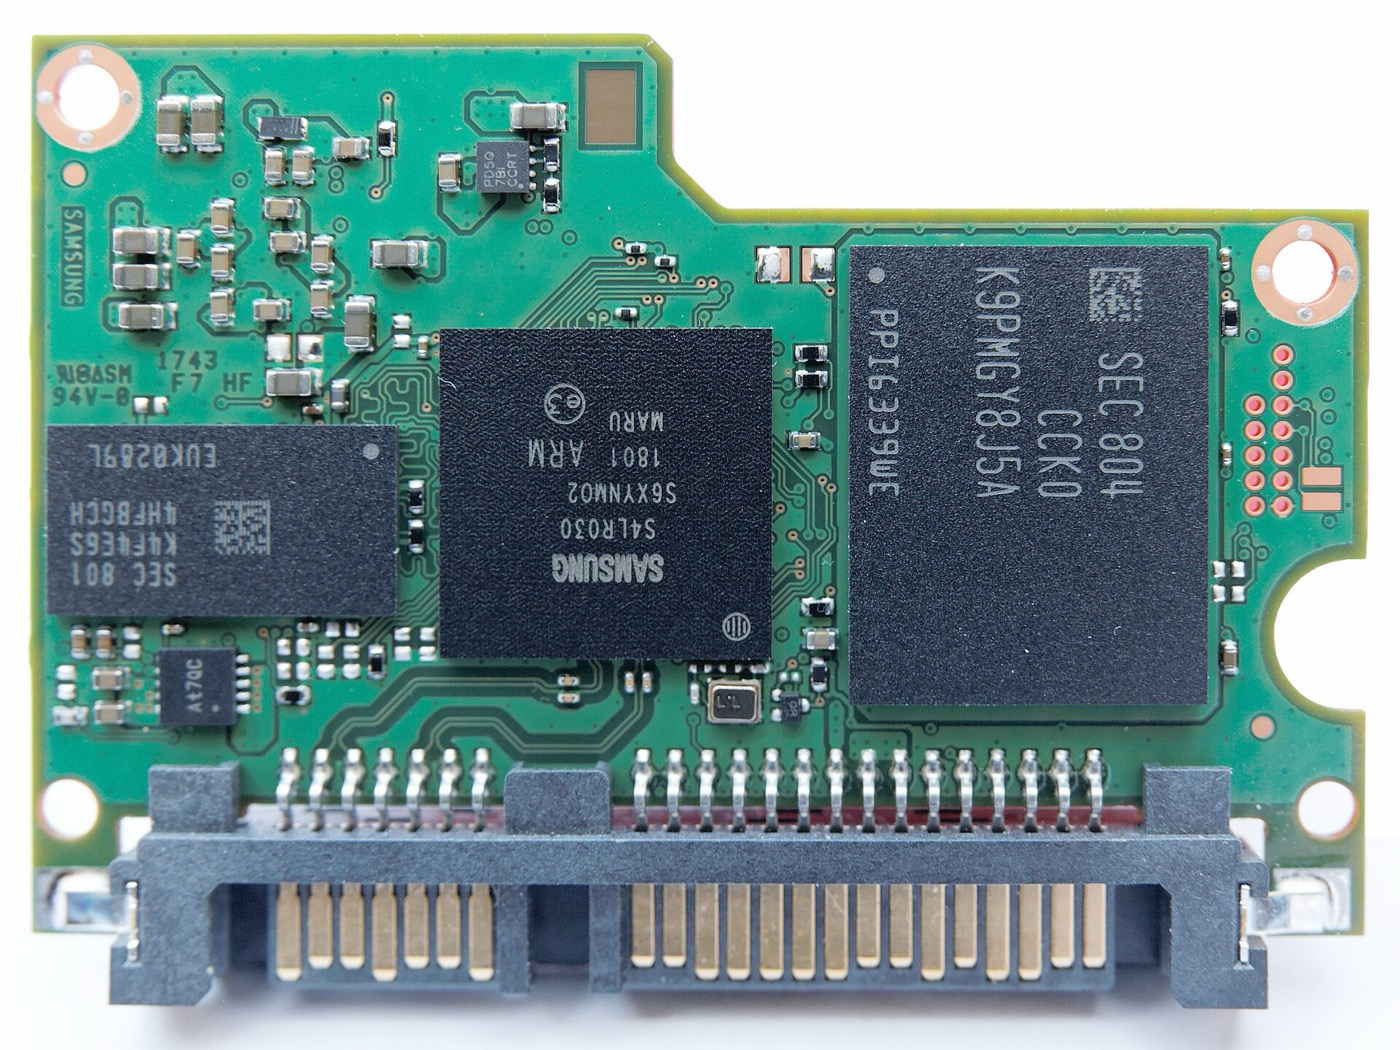
\includegraphics[width=\textwidth,height=4.6cm,keepaspectratio]{ssd_bottom.jpg}};
        \begin{scope}[x={(img.south east)},y={(img.north west)}]
          \draw[RedLine,line width=1.4pt,-{Stealth[length=6pt]}] (0.17,0.97) -- (0.17,0.62);
          \node[fill=white,text=RedLine,font=\footnotesize\bfseries,inner sep=2pt,anchor=south] at (0.17,0.92) {DRAM cache};
          \draw[darktext,line width=1.2pt,-{Stealth[length=6pt]}] (0.43,-0.02) -- (0.43,0.36);
          \node[fill=white,text=darktext,font=\footnotesize\bfseries,inner sep=2pt,anchor=north] at (0.43,-0.02) {controller};
          \draw[GreenLine,line width=1.2pt,-{Stealth[length=6pt]}] (0.80,0.97) -- (0.80,0.72);
          \node[fill=white,text=GreenLine,font=\footnotesize\bfseries,inner sep=2pt,anchor=south] at (0.80,0.92) {NAND flash};
        \end{scope}
      \end{tikzpicture}\\[0.05cm]
      {\footnotesize Failure-domain durability: name what a write survives}
    \end{column}
    \begin{column}{0.47\textwidth}
      {\footnotesize\textbf{macOS} \texttt{man 2 fsync}}\\[0.05cm]
      \codeblock{the drive itself may not physically write the data to the platters for quite some time\dots\\[0.3em]
      \textcolor{RedLine}{\textbf{This is not a theoretical edge case.}}\\[0.3em]
      F\_FULLFSYNC fcntl asks the drive to flush all buffered data to permanent storage.}
    \end{column}
  \end{columns}
  \mlsyscredit{Photo: Samsung SSD 860 Pro board, Michael Bemmerl, CC BY 3.0 de, Wikimedia Commons (labels added from the chip markings). Text: macOS 26.4 fsync(2) manual page, excerpt.}
  \note{[2 min] [CORE] Failure-domain durability: an acknowledgment is durable only against the faults its storage survives, so each write names its failure domain. The photo is a real drive. The controller accepts writes into the DRAM chip, a volatile cache, before they reach the NAND flash that keeps data without power. The manual page on the right is Apple's own: a returned fsync means only that the host handed the data to the drive; the drive may not have stored it yet. The chapter's three tiers: a process crash, survived by bytes in the kernel's page cache; power loss or a host crash, survived only after a flush that the drive honors; loss of the whole volume, survived only by copies outside it, for example two replicas acknowledged by a quorum. ENGAGE: the worksheet promises survival of host and disk together. Which tier must the intent's acknowledgment reach? (Expected: the third.) WARN: remoteness alone is not enough; an asynchronous replica can lag. FLEX: [CORE].}
\end{frame}

\begin{frame}{Predict: how long does each acknowledgment take?}
  \mlsysactivity{Predict}{2 min}
  \begin{columns}[c]
    \begin{column}{0.57\textwidth}
      \centering
      \uncover<2->{\safeimg[width=\textwidth,height=4.0cm,keepaspectratio]{acks.pdf}\\[0.05cm]
      {\footnotesize Median of \val{ack_n} appends of a \val{ack_bytes}-byte intent, one laptop SSD}}
    \end{column}
    \begin{column}{0.40\textwidth}
      \footnotesize
      \begin{tabular}{@{}P{2.05cm}P{2.75cm}@{}}\toprule
        \textbf{Survives} & \textbf{Acknowledgment} \\\midrule
        process crash & \texttt{write()} returns \\[0.05cm]
        power loss & flush the drive honors \\[0.05cm]
        volume loss & two replicas off the volume \\\bottomrule
      \end{tabular}
    \end{column}
  \end{columns}
  \mlsyscredit{Measured 2026-10-19 (images/data/ack\_latency.py): Apple M5 Max, macOS 26.4, internal SSD, APFS. Tiers: Durable Execution, \S11.3.1, table 2.}
  \note{[2.5 min] [CORE] ENGAGE: before step 2, ask for orders of magnitude: microseconds, a millisecond, ten? Step 2: measured on a laptop for this lecture, \val{ack_n} appends each. write() returned in \val{ack_write} ms, because it only copied the bytes into the kernel. fsync() returned in \val{ack_fsync} ms. F\_FULLFSYNC, which makes the drive flush its cache, took \val{ack_full} ms, \val{ack_ratio} times longer. The fast fsync is the manual page in action: it did not wait for stable media. The table maps the three tiers to the acknowledgment each needs. A replicated store adds a network round trip; the chapter's exercise uses 6.5 ms for the slower of two off-volume replicas (illustrative). Against a turn that spends seconds on the model and tools, a few milliseconds per dispatch is small. WARN: never weaken the declared domain to save milliseconds; a fast acknowledgment from the wrong tier is a durability claim that is false. FLEX: [CORE].}
\end{frame}

\begin{frame}{A missing intent proves non-dispatch only in a complete log}
  \centering
  \mlsyssteps[width=0.95\textwidth,height=5.0cm,keepaspectratio]{replica_step}{2}\\[0.05cm]
  \uncover<2->{\small Completeness rule: read absence only from a log whose prefix is proven complete.}
  \mlsyscredit{After Durable Execution, \S11.3.3 (completeness rule, table 3) and \S11.9 (pitfall).}
  \note{[2 min] [CORE] The completeness rule: the absence of a logged intent proves that no dispatch occurred only in a complete authoritative prefix of the log. Step 1: the authoritative log holds the intent for test\_r18, and the test was sent. An asynchronous replica has not yet received that entry. Step 2: a recovery routine that reads the replica sees no intent, concludes the call was never sent, and dispatches it again: a second test, or with the remediation agent a second production change. The chapter's exercise 8 prices exactly this for the remediation fleet. ENGAGE: when may recovery read a replica? (Expected: for inspection, never to decide that something did not happen.) WARN: the same holds for a diagnostic log or a cache; only the source the failure domain declares authoritative can prove absence, and only up to its first gap. FLEX: [CORE].}
\end{frame}

\begin{frame}{Group commit shares one flush; each intent still waits for all of it}
  \centering
  \safeimg[width=0.88\textwidth,height=4.4cm,keepaspectratio]{groupcommit.pdf}\\[0.05cm]
  {\small Measured: one F\_FULLFSYNC for $k$ queued intents. Chapter: \val{gc_timer} ms timer, \val{gc_flush} ms flush, \val{gc_batch} intents.}\\[0.05cm]
  {\small \val{gc_work} ms of storage work each; the first waits \val{gc_first} ms, the last \val{gc_last} ms.}
  \mlsyscredit{Measured 2026-10-19 (images/data/ack\_latency.json). Durable Execution, \S11.3.4, equation 2 (illustrative inputs). DeWitt et al., SIGMOD 1984.}
  \note{[2 min] [OPTIONAL] A runtime with many trajectories pays one acknowledgment per dispatch, and every dispatch queues at the same store. Group commit (DeWitt et al. 1984) writes several queued records with one flush. The plot is our laptop measurement: one F\_FULLFSYNC carrying \val{gc_kmin} to \val{gc_kmax} intents. The flush stays near \val{gc_flush_lo} to \val{gc_flush_hi} ms, so storage work per intent falls from \val{gc_per_hi} ms to \val{gc_per_lo} ms. The red line is what each intent waits: the whole flush. Equation 2: an intent waits its time in the queue plus the shared flush. The chapter's numbers: a \val{gc_timer} ms batch timer and a \val{gc_flush} ms quorum flush give \val{gc_work} ms of work per intent among \val{gc_batch}, but the first arrival waits \val{gc_first} ms and the last still waits \val{gc_last} ms. ENGAGE: double the timer; which term grows? (Expected: the queueing term; work per intent is unchanged if the batch size is fixed.) WARN: amortization raises throughput; it never shortens one dispatch's wait. FLEX: [OPTIONAL].}
\end{frame}

\begin{frame}{Databases log before they write; agents cannot undo the world}
  \begin{columns}[c]
    \begin{column}{0.28\textwidth}
      \centering\safeimg[width=\textwidth,height=5.0cm,keepaspectratio]{jim_gray_full.jpg}\\[0.05cm]
      {\footnotesize Jim Gray, 2006}
    \end{column}
    \begin{column}{0.68\textwidth}
      \small
      \begin{tabular}{@{}P{2.3cm}P{3.3cm}P{3.3cm}@{}}\toprule
        & \textbf{Database (ARIES)} & \textbf{Agent runtime} \\\midrule
        Logs before & writing a page & dispatching a call \\[0.05cm]
        Owns the state & yes, its pages & no, remote endpoints \\[0.05cm]
        Can undo & yes, from the log & no, compensate later \\[0.05cm]
        After a crash & redo, then undo & settle in-doubt calls \\\bottomrule
      \end{tabular}
    \end{column}
  \end{columns}
  \mlsyscredit{Photo: Microsoft Research, CC BY-SA 3.0 us, Wikimedia Commons. Gray 1978; Mohan et al., ACM TODS 1992; Helland, CIDR 2007. Durable Execution, Systems Perspective 11.1.}
  \note{[1.5 min] [OPTIONAL] Jim Gray's 1978 notes made the write-ahead log the record from which a database recovers, and ARIES (Mohan et al. 1992) turned it into a full recovery method: force the log record to stable storage before the changed page, then on restart repeat history and undo what did not commit. That works because the database owns its pages. An agent runtime logs intent for effects at endpoints it does not own. Its log can rebuild its own state, but it holds no undo for a deployment, and tools rarely offer the prepare phase of two-phase commit. Helland (2007) reached the same answer for large web systems: idempotent messages with unique identities across administrative boundaries. ENGAGE: which row explains why the hook needed an operation identity? (Expected: owns the state.) LINK: undoing an established effect is compensation, which Lecture 12 owns. Land the segment aloud. FLEX: [OPTIONAL].}
\end{frame}

% =============================================================================
% SECTION: CHECKPOINTS AND RESUME
% =============================================================================
\mlsysnote{[0.5 min] [CORE] The log protects decisions and leaves the files the agent changed unprotected, and an unbounded log grows slow to fold. Checkpoints bind both; resume turns them into authority to act.}
\mlsysdivider{How do record and files restart together, and who may act?}{Durable Execution, \S11.4 and \S11.5}
\section{Checkpoints}

\begin{frame}{A checkpoint binds record and files to one log position}
  \centering
  \mlsyssteps[width=0.95\textwidth,height=5.5cm,keepaspectratio]{ckpt_step}{3}
  \mlsyscredit{After Durable Execution, \S11.4.1 (consistent recovery boundaries; Chandy and Lamport 1985).}
  \note{[3 min] [CORE] Checkpoint binding. Step 1: a log entry saying an edit succeeded cannot restore the edited bytes. A checkpoint binds the record snapshot, record\_R\_ckpt, and the workspace snapshot, ws\_r18 (Lecture 8's copy-on-write workspace makes it cheap), to one committed log position c. Restore unpacks both and folds the suffix after c, again with no model call. Step 2: a manifest names position c, integrity hashes, and the reducer version. Publication order matters: the bytes become durable first, and only then is the manifest published; a crash mid-capture leaves the previous checkpoint in force. Step 3: the failure. Snapshot the record, then copy files a few seconds later while a tool writes: the pair describes a state that never existed, the inconsistency Chandy and Lamport's snapshot rule forbids. ENGAGE: the log points to a workspace delta whose bytes are missing. Resume? (Expected: no; fail and mark unrecoverable. Recomputing it is new execution.) FLEX: [CORE].}
\end{frame}

\begin{frame}{Full snapshots rewrite old state; deltas write it once}
  \centering
  \safeimg[width=0.88\textwidth,height=4.6cm,keepaspectratio]{snapshots.pdf}\\[0.05cm]
  {\small \val{sn_turns} turns, \val{sn_growth} KB of new state per turn: \val{sn_ratio} times the bytes written}
  \mlsyscredit{Durable Execution, \S11.4.2, equation 3 and its worked numbers (illustrative). Derived values: images/calcs.py.}
  \note{[1.5 min] [OPTIONAL] Equation 3. State grows by \val{sn_growth} KB per turn; a checkpoint every \val{sn_stride} turns gives \val{sn_n} checkpoints over \val{sn_turns} turns. A full snapshot rewrites everything accumulated so far, so total bytes grow with the square of the checkpoint count: \val{sn_full} GB. Deltas write only what changed: \val{sn_delta} MB. The ratio is (n + 1)/2 = \val{sn_ratio} for n = \val{sn_n}. The saving moves cost to recovery: restoring a delta chain means fetching, validating, and applying every delta since the base. Periodic consolidation writes a new base, and old deltas may be deleted only after that base is durably published. ENGAGE: which representation suits a trajectory that rarely crashes? (Expected: deltas, with consolidation bounding the chain.) WARN: the quadratic term comes from the snapshots; the log already appends each event once. FLEX: [OPTIONAL].}
\end{frame}

\begin{frame}{Estimate: which checkpoint stride wins on this trace?}
  \mlsysactivity{Estimate}{3 min}
  \begin{columns}[c]
    \begin{column}{0.42\textwidth}
      \begin{mlsyscard}{mlsysaccent}
        \small\textbf{Given (illustrative)}\\[0.05cm]
        \val{cd_turns} turns; crashes after \val{cd_crash_a} and \val{cd_crash_b}\\
        \val{cd_pause} s pause per checkpoint\\
        \val{cd_restore} s restore, \val{cd_rebuild} s per logged turn\\
        Strides: \val{cd_s_a}, \val{cd_s_b}, or \val{cd_s_c} turns
      \end{mlsyscard}
      \small
      \uncover<2->{Totals: \textbf{\val{cd_tot_a} s}, \textbf{\textcolor{mlsysaccent}{\val{cd_tot_b} s}}, \textbf{\val{cd_tot_c} s}\\[0.1cm]
      $k^* = \sqrt{2\delta/(\lambda r)} \approx \val{cd_k_log}$ turns\\[0.05cm]
      {\footnotesize $\delta$ pause, $\lambda$ crash rate, $r$ cost per turn}}
    \end{column}
    \begin{column}{0.55\textwidth}
      \centering\uncover<2->{\safeimg[width=\textwidth,height=5.0cm,keepaspectratio]{cadence.pdf}}
    \end{column}
  \end{columns}
  \mlsyscredit{Durable Execution, NM 11.1, equations 5 and 6 and theorem 11.1 (Young 1974). Derived values: images/calcs.py.}
  \note{[3.5 min] [CORE] Checkpoint stride. ENGAGE: two minutes in pairs; compute each total. Step 2: stride \val{cd_s_a} takes \val{cd_ck_a} checkpoints (\val{cd_cap_a} s) and rebuilds \val{cd_lost_a_a} and \val{cd_lost_b_a} turns (\val{cd_rb_a} s) plus \val{cd_crashes_words} restores (\val{cd_rest_all} s): \val{cd_tot_a} s. Stride \val{cd_s_b}: \val{cd_cap_b} s of checkpoints, \val{cd_lost_a_b} and \val{cd_lost_b_b} turns (\val{cd_rb_b} s), restores \val{cd_rest_all} s: \val{cd_tot_b} s. Stride \val{cd_s_c}: \val{cd_cap_c} s, \val{cd_lost_a_c} and \val{cd_lost_b_c} turns (\val{cd_rb_c} s), \val{cd_rest_all} s: \val{cd_tot_c} s. Checkpointing every turn would spend \val{cd_every} s, the chapter's pitfall. The plot is equation 5, from Young's 1974 balance of pause against lost work. With a crash rate of \val{cd_rate} per turn and \val{cd_rebuild} s to rebuild a logged turn, the optimal stride is about \val{cd_k_log}. If each lost turn had to be re-executed at \val{cd_reexec} s, the optimal stride is \val{cd_k_unlog}. Logging lengthens it by the square root of \val{cd_reexec} / \val{cd_rebuild}, \val{cd_gain} times, because a crash costs reconstruction instead of new model calls. WARN: the minimum is flat; a stride within a factor of \val{yg_miss} costs at most \val{yg_miss_pct} percent extra overhead, so measure before tuning. FLEX: [CORE].}
\end{frame}

\begin{frame}{A delayed worker applied an old plan and emptied a DNS record}
  \begin{columns}[c]
    \begin{column}{0.42\textwidth}
      \centering\safeimg[width=\textwidth,height=4.4cm,keepaspectratio]{ashburn.jpg}\\[0.05cm]
      {\footnotesize Data centers near Ashburn, Virginia, the region of AWS us-east-1}
    \end{column}
    \begin{column}{0.55\textwidth}
      \footnotesize DynamoDB, us-east-1, 19 to 20 October 2025, 11:48 PM to 2:40 AM (PDT)\\[0.1cm]
      \codeblock{the DNS Enactor makes a one-time check that its plan is newer than the previously applied plan\dots\\[0.3em]
      the first Enactor (which had been unusually delayed) applied its much older plan\dots\ overwriting the newer plan.}
      \textbf{\textcolor{mlsysaccent}{The check ran once, before a long delay.}}
    \end{column}
  \end{columns}
  \mlsyscredit{Quotes: AWS, Summary of the Amazon DynamoDB Service Disruption, October 2025, aws.amazon.com/message/101925. Photo: Theodore Christopher, CC0, Wikimedia Commons.}
  \note{[1.5 min] [CORE] A real incident with the zombie worker of this segment. AWS runs a DNS Planner that writes plans and three independent DNS Enactors that apply them. One Enactor checked that its plan was newer than the applied one, then stalled. Meanwhile a second Enactor applied a newer plan and began cleaning up old ones. The delayed Enactor then applied its much older plan over the newer one, and the cleanup deleted that old plan, leaving the regional endpoint with an empty DNS record. Systems that reached DynamoDB through that name failed from 11:48 PM Pacific time on 19 October until 2:40 AM the next morning. ENGAGE: where should the newer-than check have run? (Expected: at the resource, at the moment of the write.) WARN: the photo shows the region, and no building in it is identified as AWS. FLEX: [CORE].}
\end{frame}

\begin{frame}{Resume proves, owns, restores, reconciles, then admits}
  \centering
  \mlsyssteps[width=0.95\textwidth,height=4.6cm,keepaspectratio]{resume_step}{3}\\[0.05cm]
  \uncover<3->{\small Resume protocol time $=$ ownership $+$ read $+$ fold $+$ restore $+$ reconcile $+$ prefill}
  \mlsyscredit{After Durable Execution, \S11.5 and equation 7.}
  \note{[2.5 min] [CORE] The resume protocol: an authorized continuation in ordered stages; it is never a restart. Step 1: prove that the authoritative log prefix and the checkpoint artifacts are available; a gap is reported as unavailable, never read as an empty history. Then take ownership from a strongly consistent lease service, which issues a new owner epoch, 8 after 7. Step 2: restore by fold, with ws\_r18 untouched. Then reconcile: test\_r18 is in doubt, so probe the executor by its logged operation identity; budget reservations stay locked until usage evidence arrives. Step 3: only now admit new work, under current limits: a PAUSED trajectory stays paused, an approval granted before the crash still passes the dispatch-time recheck (Lecture 10's approval escrow), and bounded-liability admission (Lecture 10) runs again. Equation 7 sums the stages. ENGAGE: which stage may take longest? (Expected: reconcile or prefill; the fold is cheap.) WARN: passing the ownership check does not license re-sending test\_r18. FLEX: [CORE].}
\end{frame}

\begin{frame}{A fencing token is checked at the resource on every write}
  \centering
  \mlsyssteps[width=0.92\textwidth,height=4.6cm,keepaspectratio]{fence_step}{3}\\[0.05cm]
  \uncover<3->{\small A lease bounds how long a lost worker blocks recovery; only the epoch check excludes it.}
  \mlsyscredit{After Durable Execution, \S11.5.1 (fencing tokens; Kleppmann 2016; Burrows 2006).}
  \note{[2 min] [CORE] Fencing tokens. Step 1: worker A owns the trajectory under epoch 7, then stalls in a long pause, a network partition, or a slow disk. Its lease expires, but A does not know. Step 2: the ownership service grants epoch 8 to worker B, and B's writes to the log and dispatch gateway carry 8 and are accepted. Step 3: A wakes and writes with epoch 7. The log rejects it, because it has already seen 8. That is the check the DNS Enactor lacked: a monotonically increasing owner epoch, compared by the resource itself on every write. Burrows built the same idea into Chubby's lock sequencers. ENGAGE: A's earlier test request already reached the executor. Does epoch 8 cancel it? (Expected: no; fencing stops new writes, and test\_r18 remains in doubt until reconciled.) WARN: the fence holds only at boundaries that check it: the log, the dispatch gate, and each resource that verifies the epoch. FLEX: [CORE].}
\end{frame}

\begin{frame}{The next call after a resume prefilled \val{pf_tokens} tokens in \val{pf_cold} s}
  \centering
  \safeimg[width=0.88\textwidth,height=3.3cm,keepaspectratio]{prefill.pdf}\\[0.15cm]
  {\small Same context; the warm server kept its cached prefix. Median of \val{pf_n} runs, 7B model.}\\[0.05cm]
  {\small Chapter: \val{pf_ctx} tokens need about \val{pf_floor} s at an accelerator's 8-bit peak.}
  \mlsyscredit{Measured 2026-10-19 (images/data/resume\_prefill.py): qwen2.5 7B Q4\_K\_M on Ollama, Apple M5 Max; cold run includes \val{pf_load} s model load. Durable Execution, \S11.5.4 and \S11.9.}
  \note{[1.5 min] [OPTIONAL] The last term of equation 7. Folding the log is cheap, but the next model call needs serving state. We measured it on a laptop: a 15-turn repair transcript of \val{pf_tokens} tokens. When the same server still held the prefix from the previous turn, the next call's first token came after \val{pf_warm} s. After the model was reloaded, as on a different server, the same call took \val{pf_cold} s, about \val{pf_ratio} times longer, almost all of it prefill. The chapter's figure for its reference model and accelerator is about \val{pf_floor} s for \val{pf_ctx} tokens, as a compute floor. LINK: the radix prefix cache of Lecture 5 is what the warm server kept. The chapter's pitfall is resuming on whichever server is free. ENGAGE: when is a cold, idle server still the right choice? (Expected: when queueing at the warm one costs more than the prefill.) FLEX: [OPTIONAL].}
\end{frame}

% =============================================================================
% SECTION: REPLAY
% =============================================================================
\mlsysnote{[0.5 min] [CORE] The same records serve a second purpose that admits no new work: inspecting and testing what the trajectory already did.}
\mlsysdivider{How do we reproduce and debug a run that already happened?}{Durable Execution, \S11.6 to \S11.8}
\section{Replay}

\begin{frame}{Vote: does temperature 0 reproduce a trajectory?}
  \mlsysactivity{Vote}{2.5 min}
  \begin{columns}[c]
    \begin{column}{0.44\textwidth}
      \normalsize True or false?\\[0.2cm]
      {\small Rerunning each call at temperature 0 reproduces a recorded \val{rp_h}-turn trajectory.}\\[0.3cm]
      \uncover<2->{\textbf{\textcolor{RedLine}{False.}}\\[0.1cm]
      \small Our laptop: \val{rs_distinct0} reply in \val{rs_n0} runs.\\
      A shared server: \textbf{\val{tm_unique}} distinct in \textbf{\val{tm_n}}.\\
      Even \val{rp_q_pct}\% per call: $\val{rp_q}^{\val{rp_h}} = \val{rp_all_pct}\%$.}
    \end{column}
    \begin{column}{0.53\textwidth}
      \centering\uncover<2->{\safeimg[width=\textwidth,height=3.4cm,keepaspectratio]{feynman.pdf}\\[0.05cm]
      {\footnotesize \val{tm_n} completions at temperature 0, one 235B model}}
    \end{column}
  \end{columns}
  \mlsyscredit{He and Thinking Machines Lab, ``Defeating Nondeterminism in LLM Inference,'' 2025 (Qwen3-235B-A22B-Instruct-2507). Laptop: images/data/resample.json. Durable Execution, \S11.9.}
  \note{[2.5 min] [CORE] The chapter's third fallacy. ENGAGE: vote first. Step 2: false. On our laptop, one request at a time, \val{rs_n0} runs at temperature 0 gave \val{rs_distinct0_words} reply, the most favorable case. A serving system batches requests, and the batch changes the order of floating-point sums. Thinking Machines sampled \val{tm_n} completions of one prompt from a 235-billion-parameter model at temperature 0: \val{tm_unique} were distinct. All agreed for \val{tm_prefix} tokens, then \val{tm_major} continued ``Queens, New York'' and \val{tm_minor} ``New York City''. One flipped token changes every later token. Across a trajectory the chances multiply, Lecture 1's horizon compounding: even if each call reproduced \val{rp_q_pct} percent of the time, all \val{rp_h} would match only \val{rp_all_pct} percent of the time, before clocks, IDs, and the world change. WARN: their batch-invariant kernels made all \val{tm_n} identical, but a hosted model can also change underneath the run. Reproduction needs the recorded replies. FLEX: [CORE].}
\end{frame}

\begin{frame}{Replay substitutes recorded inputs; three modes, three answers}
  \centering
  \mlsyssteps[width=0.95\textwidth,height=5.0cm,keepaspectratio]{replay_step}{2}\\[0.1cm]
  \uncover<2->{\footnotesize\textbf{Time travel:} past state.\enspace \textbf{Regression:} new harness, old inputs.\enspace \textbf{Branch:} one change, new run.}
  \mlsyscredit{After Durable Execution, \S11.6, figure 3 and table 5 (redrawn).}
  \note{[2.5 min] [CORE] Record and replay: a sampled reply cannot be regenerated, so reproduction substitutes recorded inputs at nondeterministic boundaries. Step 1: live, every step appends to the log. Step 2: in replay the model is stubbed and tools are disconnected; recorded replies and observations stream into the harness in order. A request that matches nothing in the log stops the replay; it never falls back to a live call. Three modes use one recording. Time-travel replay folds the log to show the state at any boundary, for example what bytes reached the model at turn 18. Harness regression replay runs new harness code on the recorded inputs, with clocks and IDs captured too. A counterfactual branch restores state at a checkpoint, changes one thing, and gathers new observations in a sandbox, with production effects off and no inherited approvals. ENGAGE: a branch shows a fixed prompt succeeding once. What does that prove? (Expected: one experiment; reliability claims need task sampling, Lecture 13.) FLEX: [CORE].}
\end{frame}

\begin{frame}{Replay rejected a revised harness at its first unmatched call}
  \begin{columns}[T]
    \begin{column}{0.40\textwidth}
      {\footnotesize\textbf{Revised harness}: test before model}\\[0.05cm]
      \codeblock{\textcolor{RedLine}{\textbf{test = await workflow.}}\\
      \ind{1}\textcolor{RedLine}{\textbf{execute\_activity(}}\\
      \ind{2}\textcolor{RedLine}{\textbf{run\_tests\_keyed, ...)}}\\
      proposal = await workflow.\\
      \ind{1}execute\_activity(\\
      \ind{2}call\_model, PROMPT, ...)}
    \end{column}
    \begin{column}{0.57\textwidth}
      {\footnotesize\textbf{Replayed against the recorded history}}\\[0.05cm]
      \codeblock{NondeterminismError: [TMPRL1100] Nondeterminism error: Activity type of scheduled event 'call\_model' does not match activity type of activity command 'run\_tests\_keyed'}
      {\footnotesize The original harness replayed the same history cleanly.}
    \end{column}
  \end{columns}
  \mlsyscredit{Run 2026-10-19 for this lecture (images/data/crash\_run.py and replay.json): Temporal Python SDK 1.34.0 Replayer, history of the keyed run.}
  \note{[2 min] [CORE] Harness regression replay with a real tool. We saved the keyed run's event history and replayed it twice, with no model, no worker, and no executor. The original harness replayed cleanly. Then a revised harness that runs the test before asking the model: the first command it issued did not match the first event recorded, and the replayer stopped with the error on the right. This is the matching-request rule: every outgoing request is matched against the recording, and a mismatch fails the comparison instead of falling back to a live call. ENGAGE: is this failure a bug? (Expected: it depends on intent. A deliberate change of order is an expected divergence, and the test must declare it; an accidental one is a regression.) WARN: a passing replay proves only that the harness handles this recorded scenario; it says nothing about the agent's competence. FLEX: [CORE].}
\end{frame}

\begin{frame}{Diagnose: where did the two runs first differ?}
  \mlsysactivity{Diagnose}{2.5 min}
  \centering
  \mlsyssteps[width=0.95\textwidth,height=4.6cm,keepaspectratio]{diverge_step}{2}\\[0.05cm]
  \small Compare boundary by boundary from a verified checkpoint; stop at the first mismatch.
  \mlsyscredit{After Durable Execution, \S11.7, table 6 and the r18 example.}
  \note{[2.5 min] [CORE] First-divergence localization. The setup: a replay with a new harness ends with a different patch. ENGAGE: one minute; which boundary would you inspect first, the final patch or something earlier? Step 1: compare every boundary of every turn, in order, under a declared equivalence: the context assembled, the model reply, the harness decision, the tool observation. Turn 18 matches everywhere. At turn 19 the first boundary already differs, before any model call. Step 2: the recorded test result for r18 is identical, but a changed compaction rule (Lecture 4) dropped the note that the regression suite was omitted, while keeping the word ``passed''. Every later difference may be a consequence of that one change. WARN: the localization is a bounded claim. Whether the missing note misled the model is a separate question for a controlled branch; and equal context hashes do not prove equal requests, since decoding settings and the served model may still differ. FLEX: [CORE].}
\end{frame}

\begin{frame}{A year of recovery data costs \val{rt_share_pct}\% of one attempt}
  \centering
  \safeimg[width=0.88\textwidth,height=3.3cm,keepaspectratio]{retention.pdf}\\[0.15cm]
  {\small \val{rt_months} months at \$\val{rt_rate} per TB-month: about \val{rt_cents} cents, against a \$\val{rt_attempt} attempt}\\[0.05cm]
  {\small Recovery, replay, and diagnostics each keep their own bytes for their own time.}
  \mlsyscredit{Durable Execution, NM 11.2 (illustrative). Derived values: images/calcs.py.}
  \note{[2 min] [OPTIONAL] Recovery retention: what to keep is set by the recovery and replay promise; storage convenience does not decide it. NM 11.2: \val{rt_turns} turns of \val{rt_env} KB event envelopes and \val{rt_payload} KB of delivered inputs and results make a \val{rt_log} MB log; one \val{rt_ws} MB workspace snapshot brings it to about \val{rt_total} MB. A year at \val{rt_rate} dollars per terabyte-month costs about \val{rt_cents} cents, \val{rt_share_pct} percent of a \val{rt_attempt} dollar attempt; the log alone is \val{rt_log_pct} percent. The snapshot is \val{rt_ws_pct} percent of the bytes, so the lever is sharing workspace bases by content hash across runs of the same repository. Three lifetimes: current recovery (latest checkpoint, suffix, operation table), historical replay (older checkpoints, delivered inputs), and diagnostics (raw output, profiler traces), which Lecture 14's trace retention governs. ENGAGE: ws\_r18 is deleted but its hash survives in the manifest; can we restore? (Expected: no; a digest identifies bytes, it does not store them.) FLEX: [OPTIONAL].}
\end{frame}

% =============================================================================
% CLOSE
% =============================================================================
\begin{frame}{What the new worker should do with test\_r18}
  \mlsysactivity{Retrieval}{2 min}
  \begin{columns}[c]
    \begin{column}{0.30\textwidth}
      \begin{mlsyscard}{errorstroke}\small\textbf{The hook:} \val{rs_n} restarts from the prompt chose \val{rs_distinct} different first steps; \val{rs_tests} ran the test again.\end{mlsyscard}
    \end{column}
    \begin{column}{0.67\textwidth}
      \only<1|handout:0>{\normalsize Close your notes. List, in order, what the replacement worker does before it runs anything.}%
      \only<2->{\footnotesize
      \begin{tabular}{@{}P{0.4cm}P{7.4cm}@{}}\toprule
        1 & Prove the authoritative log is complete \\[0.03cm]
        2 & Take ownership: epoch 8, fenced at log and gateway \\[0.03cm]
        3 & Restore ws\_r18 and fold the suffix; no model call \\[0.03cm]
        4 & Probe test\_r18 by its id: job\_tests\_1 found \\[0.03cm]
        5 & Admit the next step under current limits \\\bottomrule
      \end{tabular}\\[0.15cm]}
      \uncover<3->{\footnotesize\textbf{\textcolor{mlsysaccent}{The intent was logged before dispatch, so the test was known, and its identity let one job settle the retry.}}}
    \end{column}
  \end{columns}
  \mlsyscredit{Measured runs: images/data/resample.json and summary\_RepairKeyed.json. Durable Execution, \S11.5 and \S11.10.}
  \note{[3 min] [CORE] Back to the hook. Step 1: retrieval, 60 seconds; students list the steps. Step 2: the resume protocol applied to the worksheet. The restart from the prompt sampled a new path and ran the test again. The durable runtime instead proves the log complete, takes ownership under a new epoch, restores the workspace and folds the log, which shows test\_r18 as dispatched with no result, and probes the executor by operation id; in our keyed run that found job\_tests\_1. Only then does it admit new work. Step 3: read the line. ENGAGE: what does the log still not know? (Expected: whether an in-doubt call took effect when the endpoint offers no probe, and whether a recorded action was right.) Those are the questions Lecture 12, Failure Recovery, takes up. FLEX: [CORE].}
\end{frame}

\begin{frame}{Takeaways}
  \thumbline{thumb_log.pdf}{Recovery folds an append-only log into the record; the context window cannot rebuild it.}\\[0.12cm]
  \thumbline{thumb_intent.pdf}{The intent is durable before dispatch, under a named failure domain; absence proves nothing in an incomplete log.}\\[0.12cm]
  \thumbline{thumb_cadence.pdf}{Logging each turn lengthens the optimal checkpoint stride about \val{cd_gain_round} times; resume reconciles before it admits.}\\[0.12cm]
  \thumbline{thumb_replay.pdf}{Reproduction replays recorded replies; debugging starts at the first mismatched boundary.}
  \note{[1 min] [CORE] One line per segment. Ask students which slide taught each line. If short on time, read the first two.}
\end{frame}

\begin{frame}{Open questions}
  \normalsize
  \begin{itemize}\setlength{\itemsep}{0.3cm}
    \item Many tools offer no status query and no idempotency key. Should a runtime refuse them, wrap them, or escalate every in-doubt call to a person?
    \item A hosted model can change underneath a long run. How should a runtime record what it called, when the provider does not say?
    \item Recovery data is cheap to keep, but it holds prompts, outputs, and secrets that leaked into tools. Who decides how long it lives?
  \end{itemize}
  \note{[1 min] [OPTIONAL] No single answer. The first follows from settlement before retry: without a probe or a key, an in-doubt call has no safe repeat. The second follows from the chapter's request to log available provider provenance and record its gaps. The third sets retention cost (about \val{rt_cents} cents a year) against privacy, which Lecture 14 takes up with trace retention.}
\end{frame}

\begin{frame}{Read and explore}
  \small
  \begin{itemize}\setlength{\itemsep}{0.02cm}
    \item \textbf{Read:} Durable Execution, \S11.2 to \S11.8; Checkpoints 11.1 to 11.4; Napkin Math 11.1 and 11.2 by hand; exercises 1, 3, and 8.
    \item Mohan et al., ``ARIES,'' ACM TODS, 1992: write-ahead logging and repeating history.
    \item Young, ``A First Order Approximation to the Optimum Checkpoint Interval,'' CACM, 1974.
    \item Elnozahy et al., ``A Survey of Rollback-Recovery Protocols,'' ACM Computing Surveys, 2002.
    \item Helland, ``Life Beyond Distributed Transactions,'' CIDR 2007: idempotent messages across boundaries.
    \item Burckhardt et al., ``Durable Functions,'' OOPSLA 2021: semantics of durable workflows.
  \end{itemize}
  \note{[1 min] [CORE] The chapter first, with its four checkpoints; exercise 8 prices the replica pitfall for the remediation fleet. ARIES is the complete write-ahead recovery method. Young derives the checkpoint interval. Elnozahy et al. explain why logging nondeterministic inputs changes what a checkpoint must hold. Helland explains why systems across ownership boundaries use idempotent, identified messages. Burckhardt et al. give a formal semantics for durable workflows like the one we crashed. FLEX: add the lab your course uses; the scripts in images/data rerun every measurement in this lecture.}
\end{frame}

\begin{frame}[c]
  \begin{columns}[c]
    \begin{column}{0.34\textwidth}
      \centering\mlsyskitfig[width=\textwidth,height=4.2cm,keepaspectratio]{stack_runtime}
    \end{column}
    \begin{column}{0.62\textwidth}
      {\small\textcolor{lightgray}{NEXT LECTURE \textbar{} FAILURE RECOVERY}}\\[0.5cm]
      {\LARGE\bfseries The log records every step. Why can a recovered run still leave the world half changed?}
    \end{column}
  \end{columns}
  \note{[0.5 min] [CORE] Today kept the record. Lecture 12 decides what to do with what the record cannot settle: retries an endpoint permits, compensations registered before the effects they undo, and watchdogs for runs that fail without raising an error.}
\end{frame}

\end{document}
